\documentclass{beamer}
\usepackage{ctex} % To support Chinese characters, if needed
\usepackage{graphicx} % To include images
\usepackage{hyperref} % To include hyperlinks
\usepackage{amsmath} % For mathematical symbols
\usepackage{booktabs} % For beautiful tables

% Theme choice:
\usetheme{Madrid}
\usecolortheme{seahorse}

% Custom block colors
\setbeamercolor{block title}{bg=blue!30,fg=black}
\setbeamercolor{block body}{bg=blue!10,fg=black}
% \setbeamercolor{alertblock title}{bg=red!50,fg=white}
% \setbeamercolor{alertblock body}{bg=red!20,fg=black}
\setbeamercolor{exampleblock title}{bg=green!50,fg=black}
\setbeamercolor{exampleblock body}{bg=green!20,fg=black}

% Enable figure numbering
\setbeamertemplate{caption}[numbered]


% Title, author, and date information:
\title{\textbf{Learning Research}}
\author[xjh]{Jiahao Xiang\inst{1}}
\institute{
    \inst{1}
    Hengyang Normal University
}
\date{\today}

\begin{document}

\begin{frame}
    \titlepage
\end{frame}

\begin{frame}
    \frametitle{Preface}
    % introduce the share speech motivation
    \textbf{Motivation:} 对于接触Research一年多,还是小白的我来说,不具备一套高效的方法论。这次分享,我们对常年混迹与顶会的,一位浙大的大佬(彭思达)分享的\texttt{learning\_research}进行学习,在大佬的输入下,输出一下我们学习到的内容,希望能够对大家也有所帮助。
    \vfill
    \begin{block}{大佬思想使用该颜色块标注}
        \url{https://github.com/pengsida/learning_research}
    \end{block}
    \begin{exampleblock}{我们的想法}
        汇报 slide: \url{https://github.com/jiahaoxiang2000/TempWrite/blob/master/slied/learning_research.pdf}
    \end{exampleblock}
    
    
\end{frame}

\begin{frame}
    \frametitle{Table of Contents}
    \tableofcontents
\end{frame}

\section{找问题}
\begin{frame}
    \frametitle{找问题}
    \begin{block}{一阶段}
        这个阶段追求\textcolor{blue}{广度},了解一些基础的概念和算法。不要求深度,不要求掌握/熟悉算法所有的细节。这个阶段的目的是让你对大方向有一个大概的了解,知道有哪些算法,知道这些算法的\textcolor{blue}{大概原理},知道这些算法的应用场景。
    \end{block}
    \begin{block}{二阶段}
        这个阶段追求\textcolor{blue}{深度},追求掌握某一篇论文的细节(算法细节、代码实现细节)。这个阶段的目标是构建某一个科研细分方向的算法基础,了解一篇\textcolor{red}{论文}是怎么做出来的(寻找科研问题、想idea、做实验、写论文)。
    \end{block}
    \begin{exampleblock}{找问题}
        当来到二阶段时,一类问题已经明显了,一类为旧的issue,我们阅读的文献;二类为新的issue,属于开创新的贡献。
    \end{exampleblock}

\end{frame}

\section{解问题}
\begin{frame}
    \frametitle{解问题}
    \begin{block}{三阶段}
        在有了一定算法基础以后,开始在实验室的指导下做一个自己一作的Project。这个阶段的目标是通过\textcolor{red}{实践}来学习一篇论文是怎么做出来的。
    \end{block}
    \begin{exampleblock}{想idea}
        想点子的过程,就是尝试去解问题的过程。找找旧的解法,看看有没有可以改进的地方,或者能不能引入一些新的思路。
    \end{exampleblock}
    \begin{block}{杨植麟认为}
        技术的本质就是对方法做\textcolor{red}{组合},把小的技术组合成大的技术,把老的技术组合成新的技术。
    \end{block}
\end{frame}

\begin{frame}
    \frametitle{想idea}
    具体的想idea的流程(Goal-driven research)
    \begin{block}{1. general goal}
        一般而言,general goal容易定义,但制定roadmap需要对领域有深刻的理解。可以通过构建literature tree来建立起对该领域的认知。
    \end{block}
    \begin{block}{literature tree}
        \begin{itemize}
            \item 收集相同方向的论文。
            \item 通过阅读论文,梳理出当前方向已有的milestone tasks,并标记提出该\textcolor{red}{task}的第一篇论文(1类novelty)。
            \item 将论文根据milestone tasks进行归类。梳理出有代表性的pipelines,并标记提出该\textcolor{red}{pipeline}的第一篇论文(2类novelty)。
            \item 根据pipeline再细分到novel \textcolor{blue}{module},归类论文(3类novelty)。加一些module改进已有pipeline地工作 (4类novelty)
            \item 随着自己对领域的理解,增加新的milestone tasks。
        \end{itemize}
    \end{block}
\end{frame}

\begin{frame}
    \frametitle{想idea}
    \begin{exampleblock}{novelty的分类}
        创新性越高,它所能影响的文章数量就越多。1类milestone task,2类novel pipeline,3类novel module,4类旧module改进已有pipeline地工作。i.e. \textcolor{blue}{创新性很大程度上,影响文章录用的level。}
    \end{exampleblock}
    \begin{block}{2. 选题}
        根据novelty-tree列出的roadmap,选择有研究空间的task,调研这个task有没有重要的technical challenge。\textcolor{red}{选题是对一个research project影响最大的一步,而不是后面的想方法。}
    \end{block}
    \begin{block}{3. why not work reason?}
        从技术层面上分析现在的pipelines在某个task上不work的原因,在pipeline module层面思考可能的原因,然后在pipeline层面或high-level idea层面思考可能的原因。
    \end{block}

\end{frame}

\begin{frame}
    \frametitle{想idea}
    \begin{block}{4. Innovation}
        \begin{itemize}
            \item 通过看论文、思考、做实验、与人讨论等方式,发现当前的pipeline满足不了哪个指标。找到的“问题”。
            \item 1)寻找有没有解决相似“问题”的论文,看看这些论文里有没有分析导致“问题”的技术原因。2)从论文获得的知识。总结这些论文的分析,形成自己的一套思考。3)从有经验的人身上蒸馏知识。4)从实验获得知识。
        \end{itemize}
    \end{block}
    \begin{exampleblock}{找点子}
        点子函数$f:g\mapsto q$, 其中$g$为具有泛化性的知识,i.e. 可以用在多个问题上,$q$为具体的问题。我们的目标是找到一个函数$f$,使得$q$尽可能优。

        1)知$f_1:g\mapsto q_1,q_1\approx q_2$,求$f_2:g\mapsto q_2$。2)和3)知$q$,找$g$,求$f$。4)知$q,g$,求$f$。\textcolor{blue}{2)和3)难,1)简单一些}。
    \end{exampleblock}
    5. 实验验证创新点。
\end{frame}

\begin{frame}
    \frametitle{想idea}
    \begin{block}{Goal-driven research在research产出方面的好处}
        Goal-driven research的风格是追求重要的任务,试各种方法把这个任务做work。通过一些条件的relax,总可以把一些重要的任务做出一些work的结果。这样project有\textcolor{red}{产出的保证}。

        有些人喜欢追新技术,一味的把新技术调work。但我们这方向是实验科学,不通过大量实验难以确定一个技术是否真的work,导致这种科研方式风险性太大了。
    \end{block}
    \begin{block}{当出现新锤子的时候}
        非常值得拿新锤子来做自己roadmap上的某一个milestone task,这样容易做出有影响力的工作。如:
        \begin{itemize}
            \item Transformer出来的时候,拿来搞LoFTR
            \item NeRF出来的时候,拿来搞Neural Body
            \item Stable diffusion出来的时候,拿来搞DreamFusion、DreamBooth
        \end{itemize}
    \end{block}
\end{frame}

\begin{frame}
    \frametitle{想idea}
    \begin{block}{实验室的帮助}
        \begin{itemize}
            \item 开箱自带重要的科研问题 task。
            \item 丰富的Review经验。
            \item 防止进入local minimum,路走窄。
            \item 避免technical flaw,路走死。
            \item 帮改进其提出的创新。
        \end{itemize}
    \end{block}
\end{frame}


\section{做实验}

\begin{frame}
    \frametitle{做实验}
    \begin{figure}[h]
        \centering
        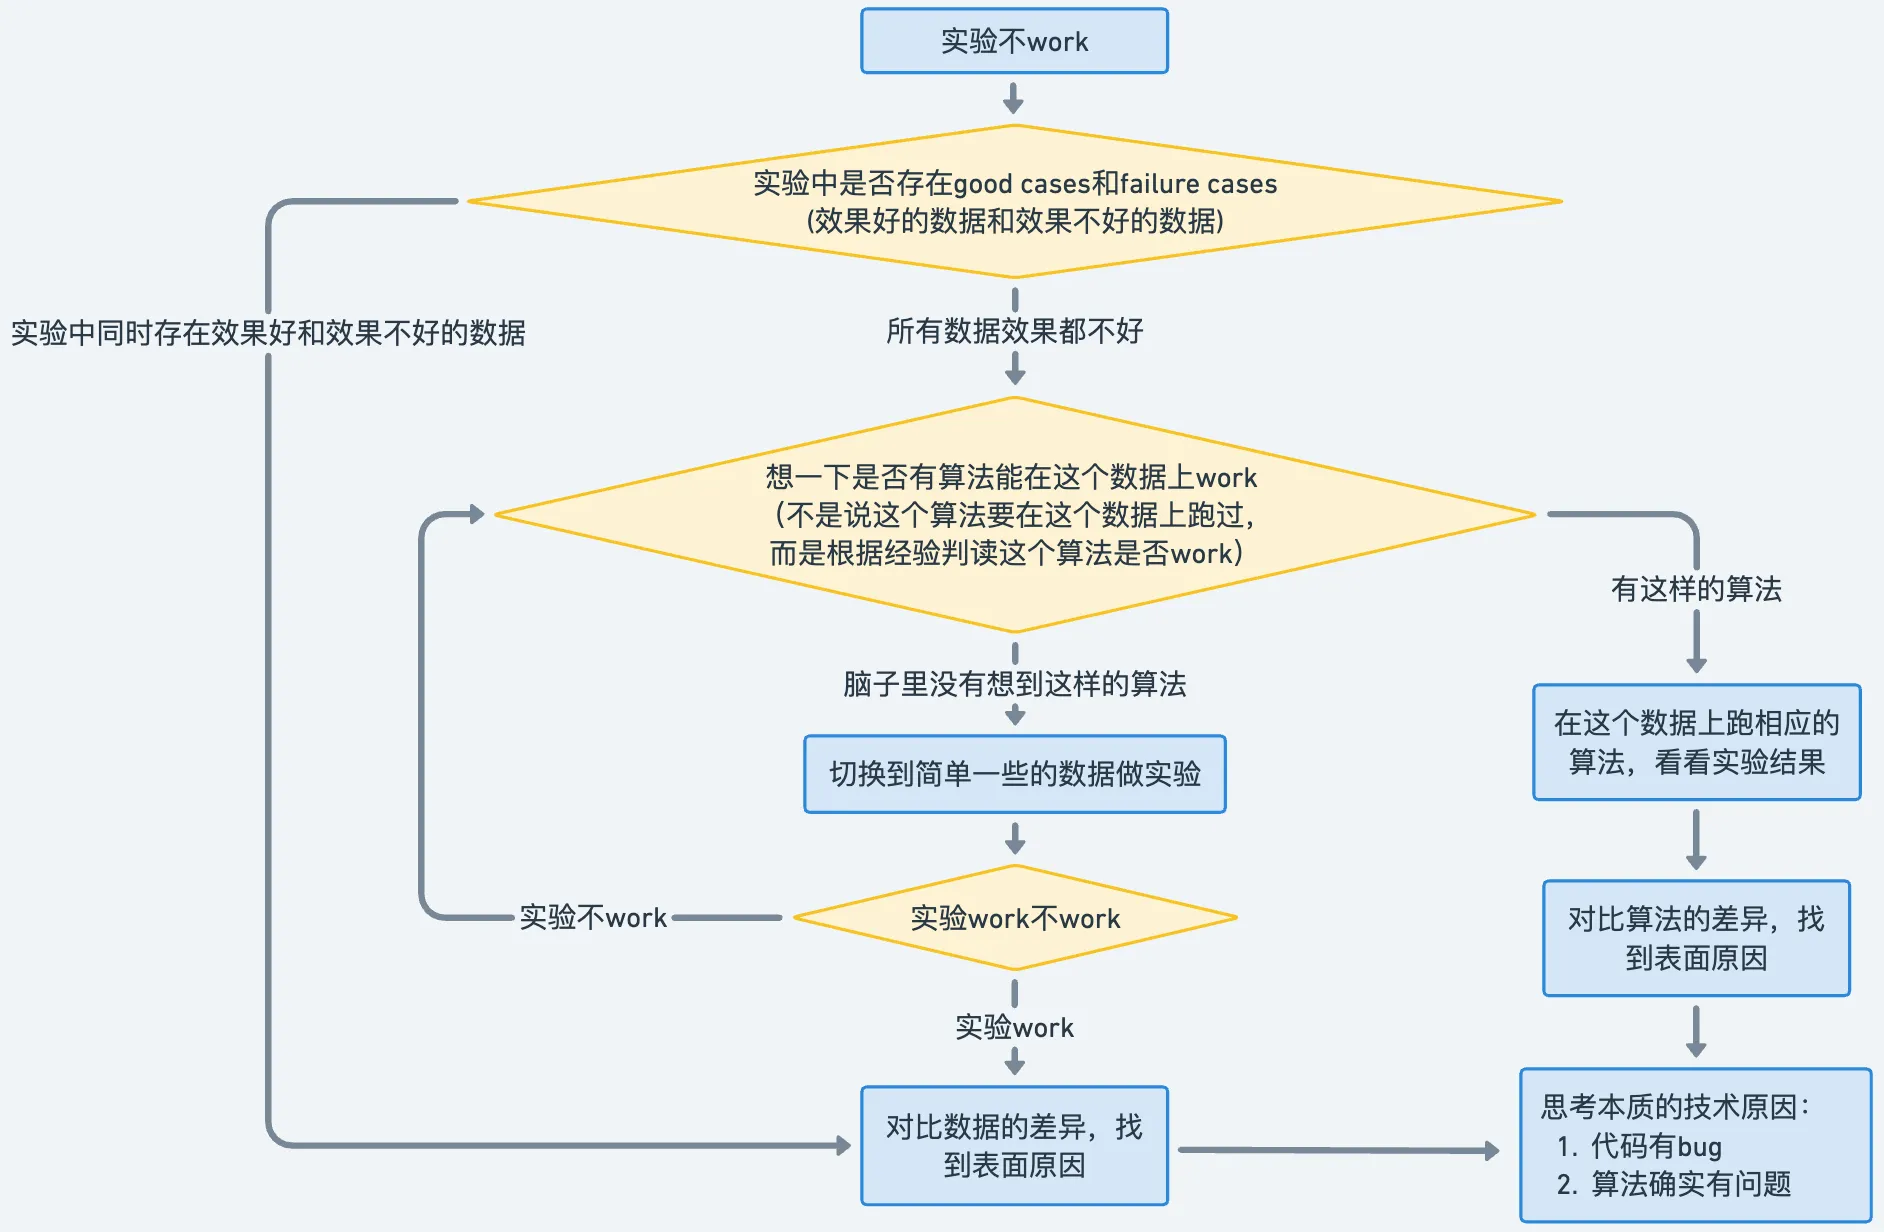
\includegraphics[width=0.8\textwidth]{figure/idea_not_work.png}
        \caption{如何找到当前实验不work的原因}
        \label{fig:experiment}
    \end{figure}
\end{frame}


\begin{frame}
    \frametitle{做实验}
    \begin{block}{not work怎么办}
        \begin{enumerate}
            \item 搜集当前实验的failure cases
            \item 搜集当前实验的good cases(效果好的实验结果),或者找到一个能work的实验版本。方式:\textcolor{blue}{降低问题复杂度,遍历问题点。}
            \item 分析“work的实验版本”和“不work的实验版本”之间存在performance gap的技术原因。\textcolor{red}{列出尽量多的技术原因。}
            \item 实验验证上一步中提出的技术原因。\textcolor{red}{快速迭代。}
            \item 针对导致failure cases的技术原因,提出解法。(需要建立自己的武器库,知道学术界都有哪些技术。可以通过构建\textcolor{blue}{literature tree}来帮助建立武器库。)
            要经常性地确认自己在正确的方向上:当前的算法思路真的对吗。要避免陷入local minima。建议经常找同学\textcolor{blue}{交流讨论}。
        \end{enumerate}
    \end{block}
\end{frame}

\section{写论文}
\begin{frame}
    \frametitle{写论文}
    \begin{block}{写论文的步骤}
        \begin{itemize}
            \item 画一个清楚的pipeline figure的草图(\textcolor{blue}{理清楚方法}的流程步骤)。
            \item \textcolor{blue}{梳理论文的story}(倒推,然后正推。详细做法见Introduction部分)。整理成story以后,写一个introduction的思路。同时列出要做的comparison experiments。
            \item \textcolor{blue}{写method,同时做实验。}
            \item 改introduction和method,同时做实验。
            \item 实验做差不多以后,写experiment。
            \item 写related work。
            \item Review论文。改论文的introduction、method和experiment。
            \item 写abstract,取论文名字。
            \item \textcolor{blue}{反复review论文,改论文。}
        \end{itemize}
    \end{block}
\end{frame}

\begin{frame}
    \frametitle{写论文}
    \begin{block}{把论文做得漂亮、美观,让人第一印象觉得这篇论文很高级。}
        \begin{itemize}
            \item 好看的teaser figure、pipeline figure。
            \item 好看的表格和结果图。
            \item 整齐的排版。
        \end{itemize}
    \end{block}
    \begin{block}{段落写作原则}
        \begin{itemize}
            \item 一段文字只讲\textcolor{blue}{一个Message},并表达清楚,不要把几个Messages杂糅在一起。
            \item 一段文字开头\textcolor{red}{第一句}就要让读者知道这段在说什么。
        \end{itemize}
    \end{block}
    \begin{block}{\textcolor{red}{Flow},WILLIAM ZINSSER,On Writing Well}
        \textit{Good writing have an aliveness that keeps the reader reading from one paragraph to the next.}
    \end{block}
\end{frame}

\section{Conclusion}

\begin{frame}
    \frametitle{Conclusion}
    \begin{exampleblock}{回顾}
        \begin{itemize}
            \item 找问题:广度、深度、新问题、旧问题。
            \item 解问题:goal-driven research、找点子。
            \item 做实验:not work怎么办。
            \item 写论文:写作步骤、写作原则。
        \end{itemize}
    \end{exampleblock}
\end{frame}

\begin{frame}
    \frametitle{Advise}
    \begin{block}{Advise Form Bill Freeman}
        \begin{itemize}
            \item "Slow down to speed up", It may feel like you’re going slowly, but you’ll be making much more progress than if you flail around, trying different things, but not understanding what’s going on.
            \item "How do I get myself to work hard enough to do research well?" You become good at it because you spend time at it and you do that because you enjoy it.  If you’re not the type who falls in love with a problem, then just know that working hard is what you have to do to succeed at research.
            \item Sometimes it’s useful to think that everyone else is an idiot. This lets you do things that no one else is
            doing.
            \item I love to hear about progress when I meet with students, but note that I have a very general notion of
            progress. Progress can include: “I’ve shown why this doesn’t work”, “I’ve simplified the task to get it to
            start working.”.
        \end{itemize}
    \end{block}
\end{frame}

\begin{frame}
    \frametitle{THANK YOU}

    \begin{block}{}
        \begin{center}
            \Huge{感谢大家的时间!}
            % last insert one home page figure, then talk, if have any question please ask me.
        \end{center}
    \end{block}
    \begin{figure}[h]
        \centering
        
\includegraphics[width=0.4\textwidth]{figure/qrcode_www.yuque.com.png}
        \label{fig:home_page}
    \end{figure}
    \small{以上是我们的个人主页,大家有什么问题可以随时联系我们。}
\end{frame}

\end{document}